\section{Conclusion}
\label{sec:conclusion}

\subsection{Summary}

We presented a multimodal ensemble system for presurgical brain tumor classification. Our approach combines a dual-path neural network with cross-modal gating (report + tabular) with gradient-boosted tree models (XGBoost, LightGBM, CatBoost), achieving \textbf{86.98\%} Micro-F1 on 5-fold OOF validation with the submission weights, and 87.25\% with grid-search-optimal weights.

Key findings:
\begin{enumerate}
  \item \textbf{Radiology reports dominate} (84.29\% alone vs 46.6\% baseline). The radiologist's narrative integrates all imaging findings into a single informative signal.
  \item \textbf{Raw radiomics are near-useless} (52.21\%, barely above baseline). Global texture statistics do not capture clinically relevant patterns.
  \item \textbf{Robustness to distribution shift is a first-class concern.} We incorporate hierarchical location encoding, missing flags, BERT semantic embeddings, and ensemble diversity as generalization-promoting strategies, though their effectiveness cannot be confirmed without labeled out-of-distribution data.
  \item \textbf{NN-dominant weighting is a hypothesis for robustness} at the cost of 0.27\% OOF. BERT embeddings may generalize better under shift than tree model thresholds, but this remains unverified without test labels.
  \item \textbf{Ensemble diversity requires different input signals.} Three GBT algorithms on the same features show only 0.58\% spread; true gains come from combining text (NN), tabular (MLU), and probability (NNXGB) signals.
\end{enumerate}

\subsection{Final Performance}

\begin{figure}[H]
\centering
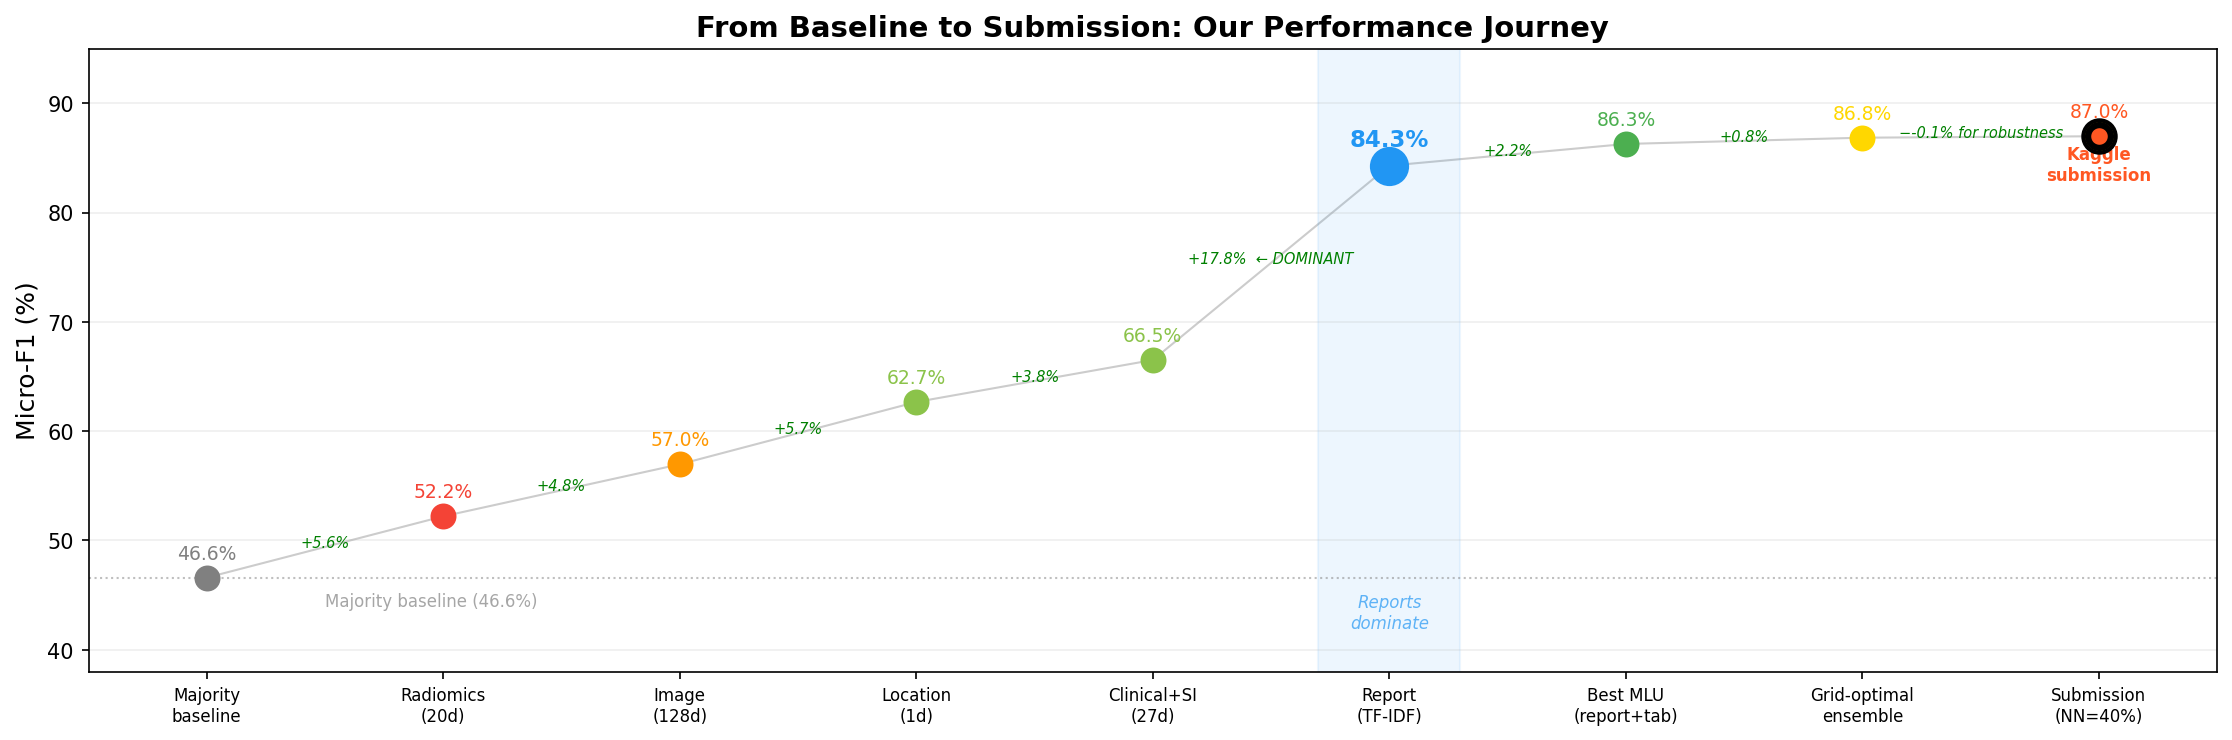
\includegraphics[width=\textwidth]{figures/final_summary.png}
\caption{From baseline to final ensemble: progression of Micro-F1 scores. The report solo turning point at 84.3\% provides the dominant signal. Adding tabular features (+2.2\%) and a 6-model ensemble (+0.8\%) brings the grid-search optimal to 86.9\%. The submission configuration achieves 87.0\% with NN-dominant weighting (40\%).}
\label{fig:final_summary}
\end{figure}

\begin{table}[H]
\centering
\caption{Final model summary. Data from model\_final.ipynb Cells 20, 25--27.}
\label{tab:final_summary}
\begin{tabular}{lcc}
\toprule
\textbf{Component} & \textbf{Description} & \textbf{Result} \\
\midrule
Solo best & MLU-XGB (TF-IDF + Tabular) & 86.28\% Micro-F1 \\
Neural Network & BERT dual-path + CrossModalGate & 82.35\% Micro-F1 \\
Ensemble (grid-optimal) & 6 models, grid-search weights & 87.25\% Micro-F1 \\
Ensemble (submission) & 6 models, NN-dominant (40\%) & \textbf{86.98\% Micro-F1} \\
\midrule
Macro AUC (ensemble) & Ensemble & 96.4\% \\
\bottomrule
\end{tabular}
\end{table}

\subsection{Reproducibility}

All experiments are reproducible (model\_final.ipynb + ML\_experiments.ipynb):
\begin{itemize}
  \item Fixed random seeds (\texttt{random\_state=42})
  \item PCA and TF-IDF fitted on training data only
  \item CLS token for BERT (not mean pooling)
  \item Complete pipeline in two notebooks
\end{itemize}

\subsection{Tools}

AI-assisted tools were used for code debugging and figure visualization. All experimental design, model architecture decisions, and analysis were conducted by the authors.
